\chapter{{\tt Stereo} Module}
\label{ch:stereo-module}

Stereo module's focus is finding a dense correlation between two
images taken of the same object from different locations. Dense
correlation means that every pixel in the first image has been
correctly matched to a pixel in the second image.

This dense matching is useful for recreating an ability every human
has and that is stereo vision. Using Camera Models discussed in Camera
Module and using a dense correlation solved for in this module, a 3D
measurement can be created for every pixel. This has use in rover
navigation, as it allows for the land ahead to measured for steepness
and roughness of terrain. It can also be used for the construction
topographical maps created from satellite imagery that allows for
measurement of every mountain, canyon and crater.

The following chapter is order mostly in the fashion that 3D models
are created. We'll start with a discussion of the storage format for a
dense correlation called a disparity map. Then we'll cover solving for
a rough integer estimate of a disparity map in Stereo
Correlation. Next is finding the floating point solution of that
disparity map call Subpixel Refinement. Finally we'll discuss the code
that converts all of this data into 3D measurement with
StereoView. We'll also point you to a demo tool that uses the
discussed code.

\section{Disparity Maps}
\label{sec:disaprity_maps}

As mentioned before a disparity map is the data structure that we use
to store the solution of the dense correlation. Simply it's just an
{\tt ImageView<PixelMask<Vector2f> >}. Disparity Maps are always
associated with a left and a right image. Given a $I_L(x,y)$ in the
left image, it's correspond index in the right image is found with
$Il_Lx,y) + D(I_L(x,y)) = I_R(x,y)$, where D is the disparity
map. Pixel Mask is used to keep track of failures that is usually
caused by an unstable solution or saturation of the input image (like
a shadow or highlights). Figure \ref{fig:disparity-example} is an
example of what a typical disparity map looks like created from images
that were aligned before feeding to the {\tt correlate} tool.

\begin{figure}[bp]
\centering
  \subfigure[{\tt Left Image}]{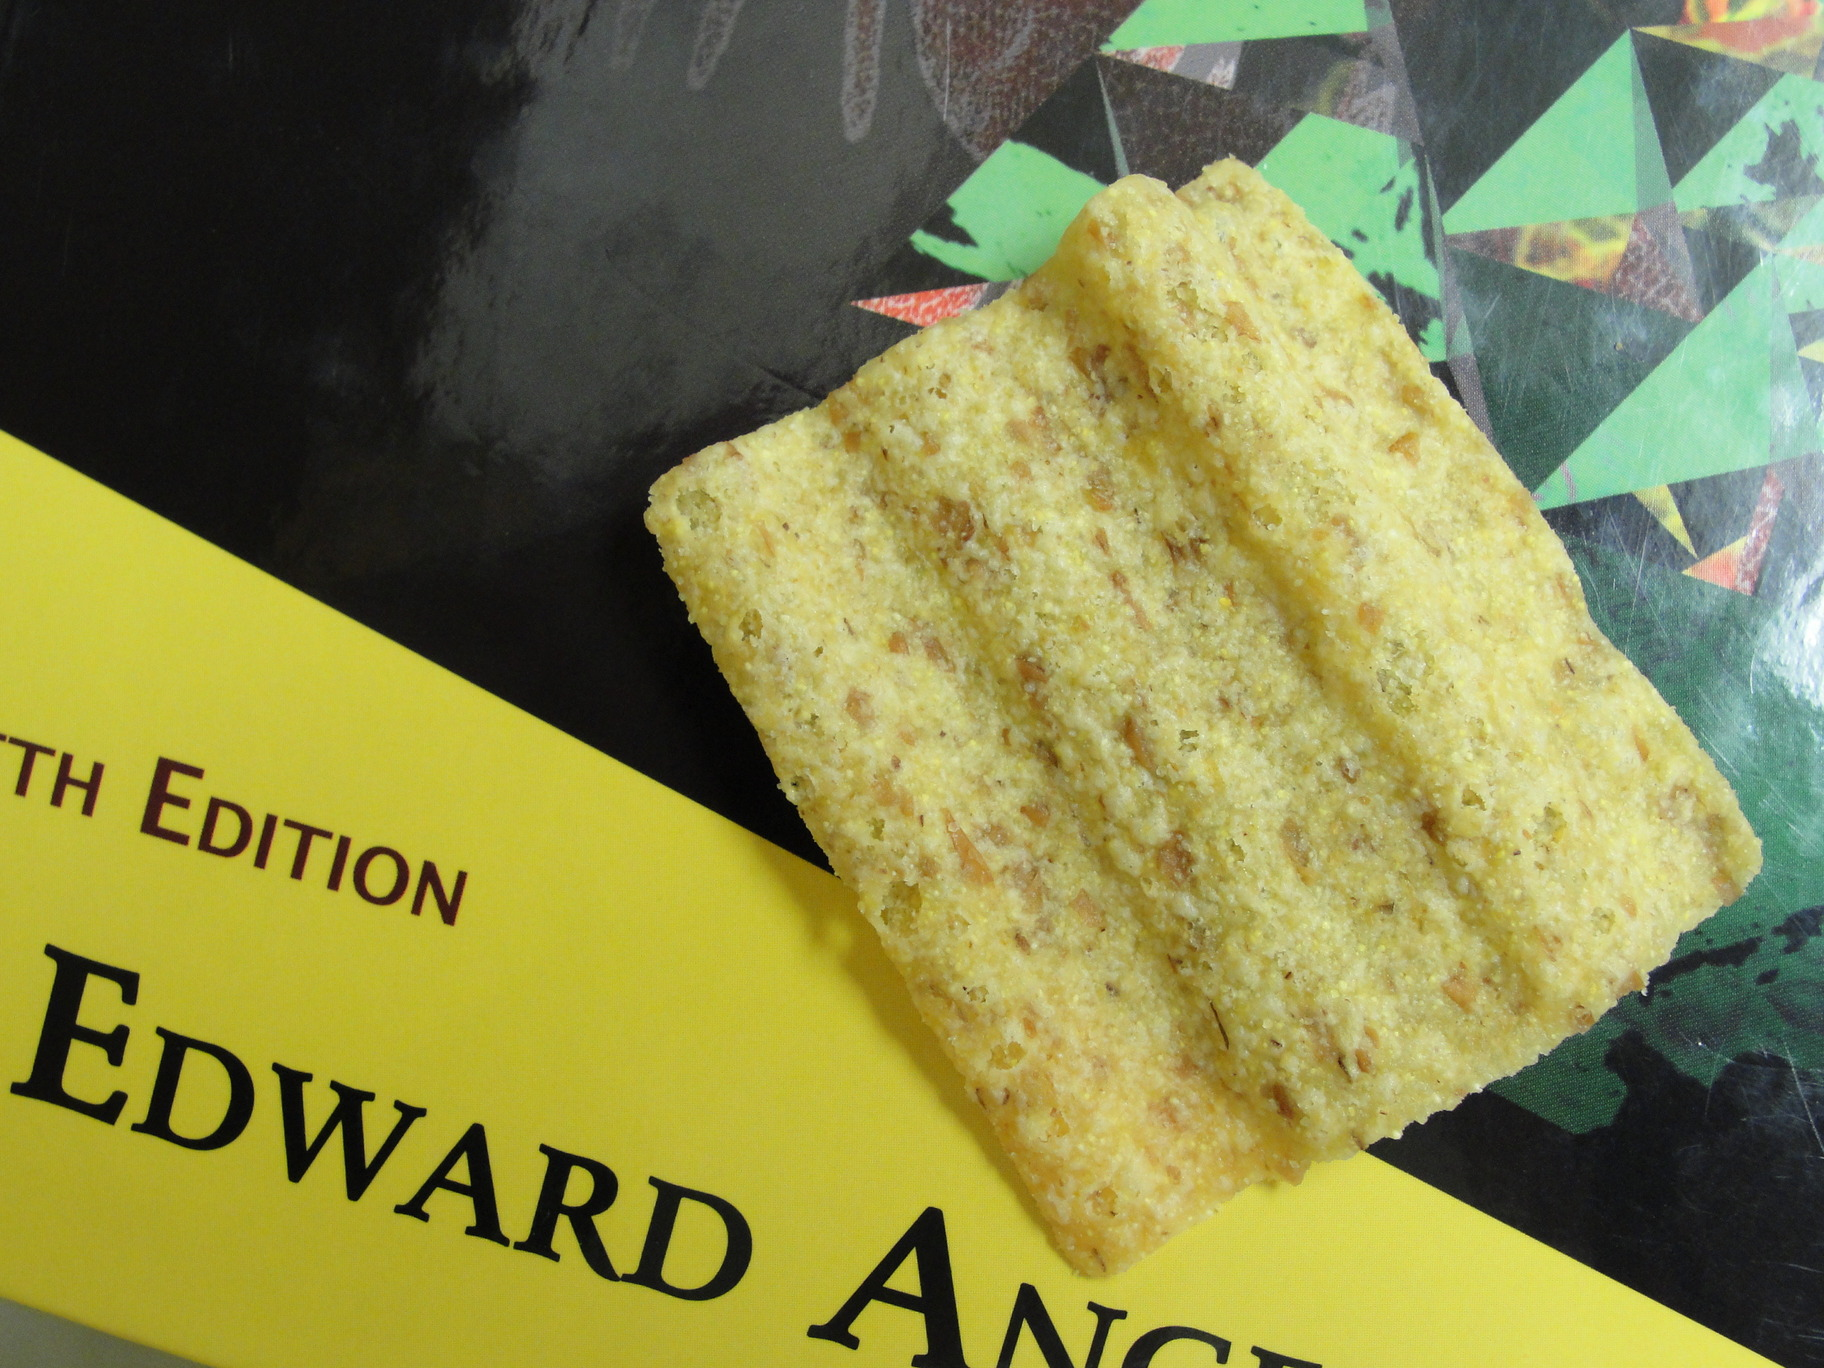
\includegraphics[width=3in]{images/stereo/left.jpg}\label{fig:disp-ex-left}}
  \hfill
  \subfigure[{\tt Right Image}]{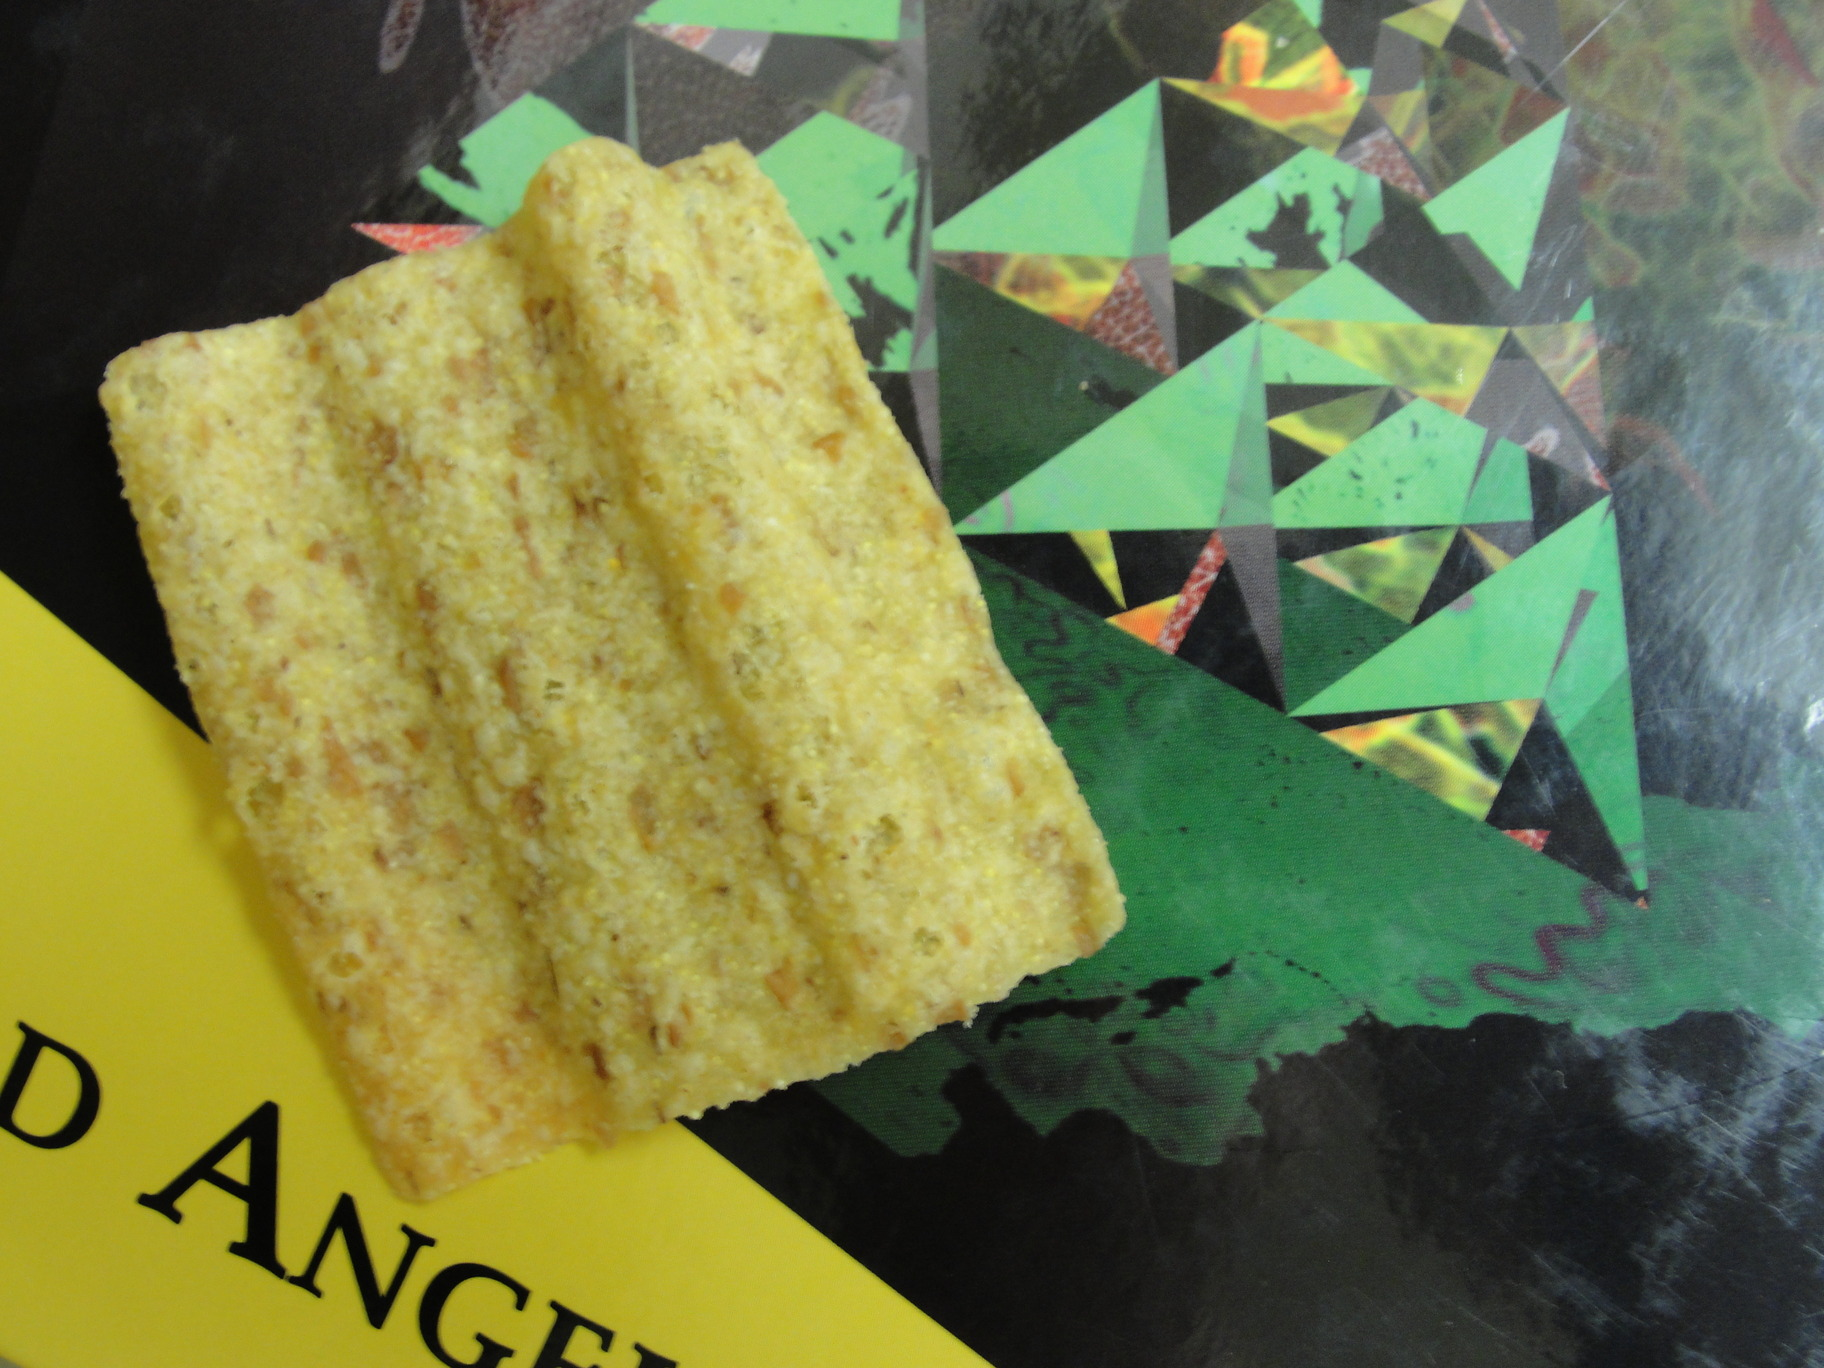
\includegraphics[width=3in]{images/stereo/right.jpg}\label{fig:disp-ex-right}}
  \\
  \subfigure[{\tt Disparity Ch:0} \emph{Horizontal offset}]{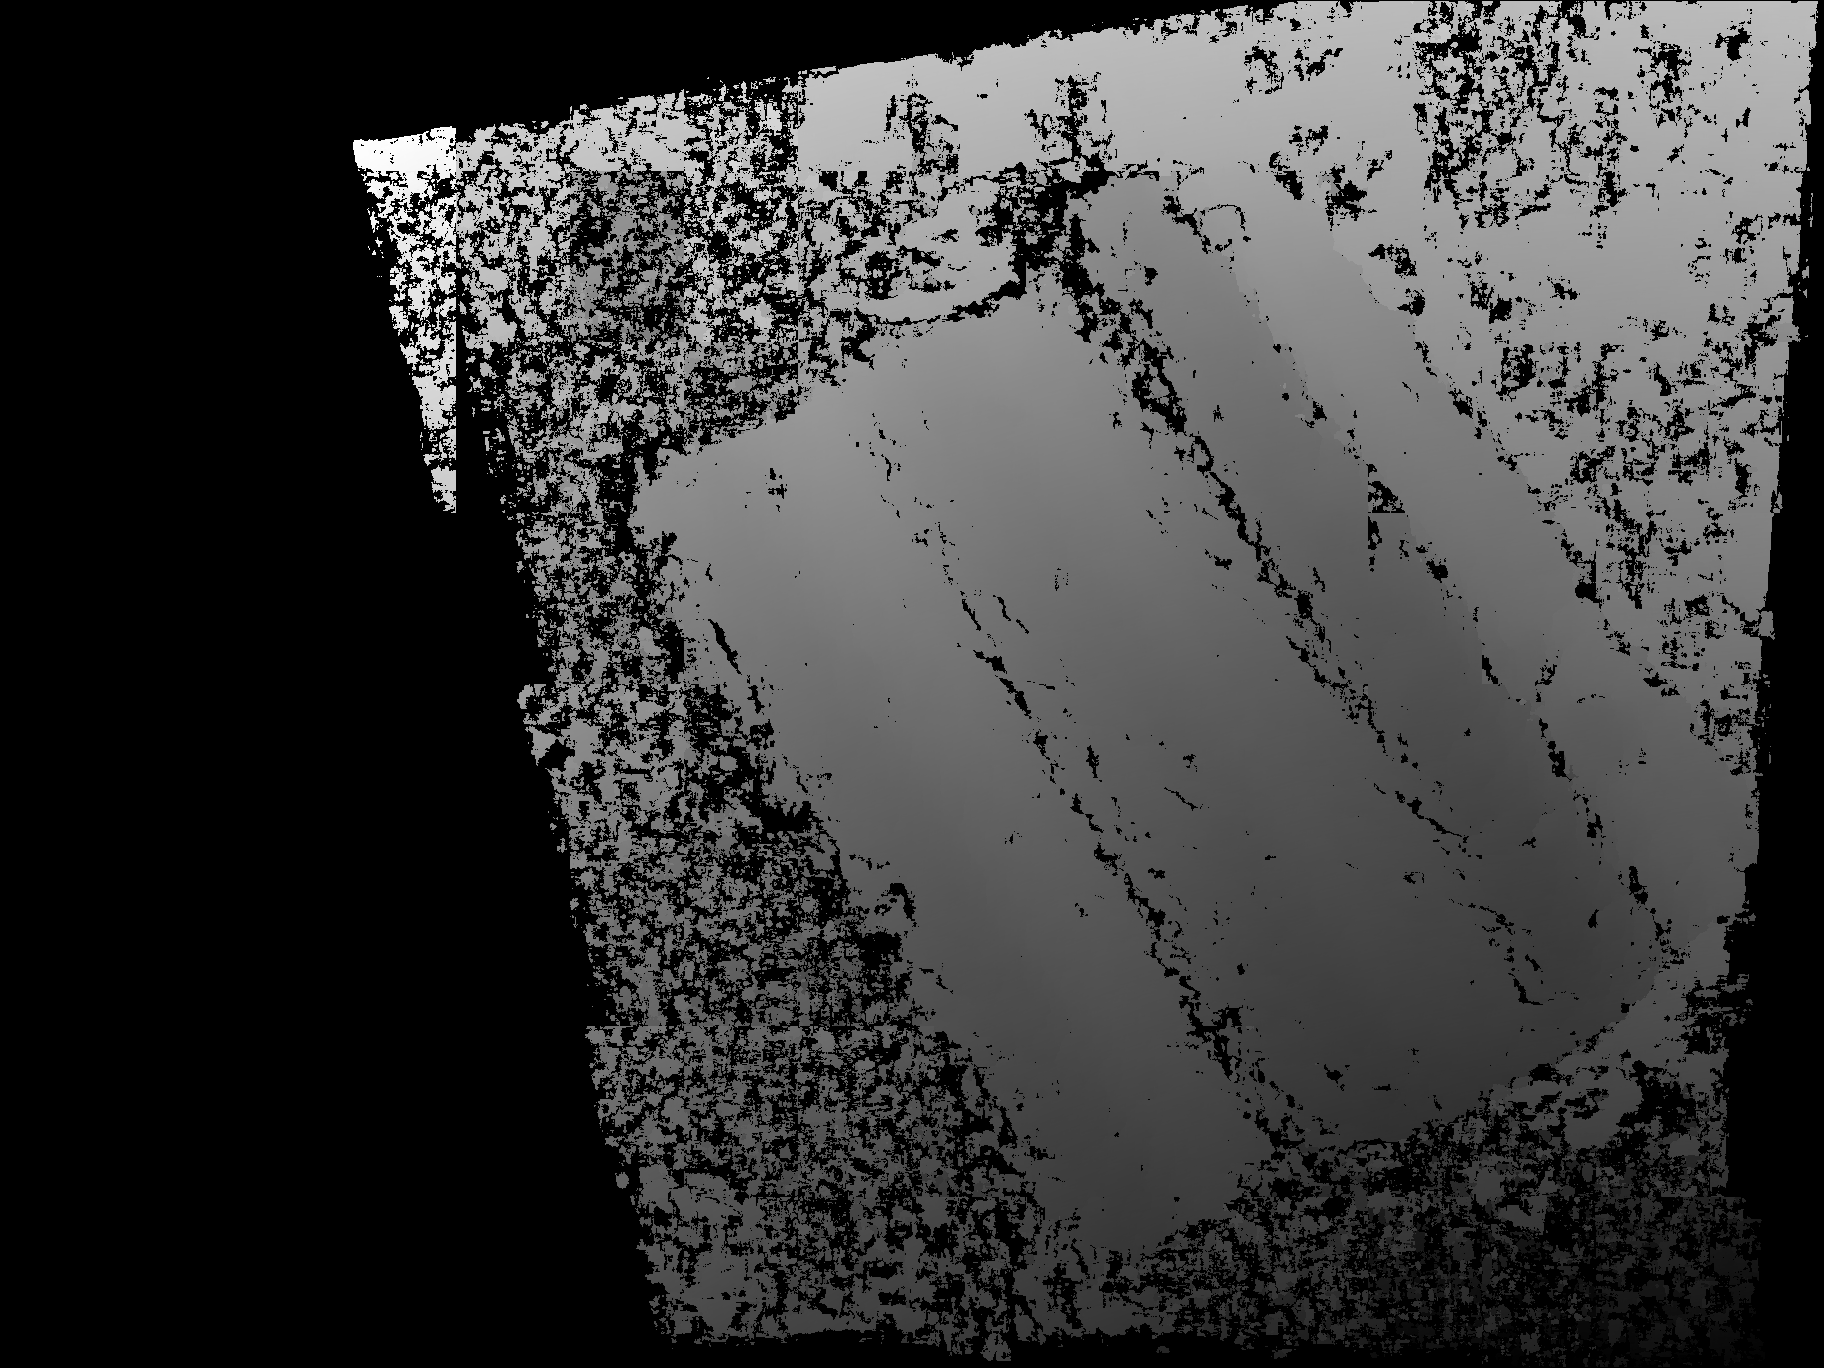
\includegraphics[width=4in]{images/stereo/x_disparity.png}\label{fig:disp-ex-ch0}}
  \\
  \subfigure[{\tt Disparity Ch:1} \emph{Vertical offset}]{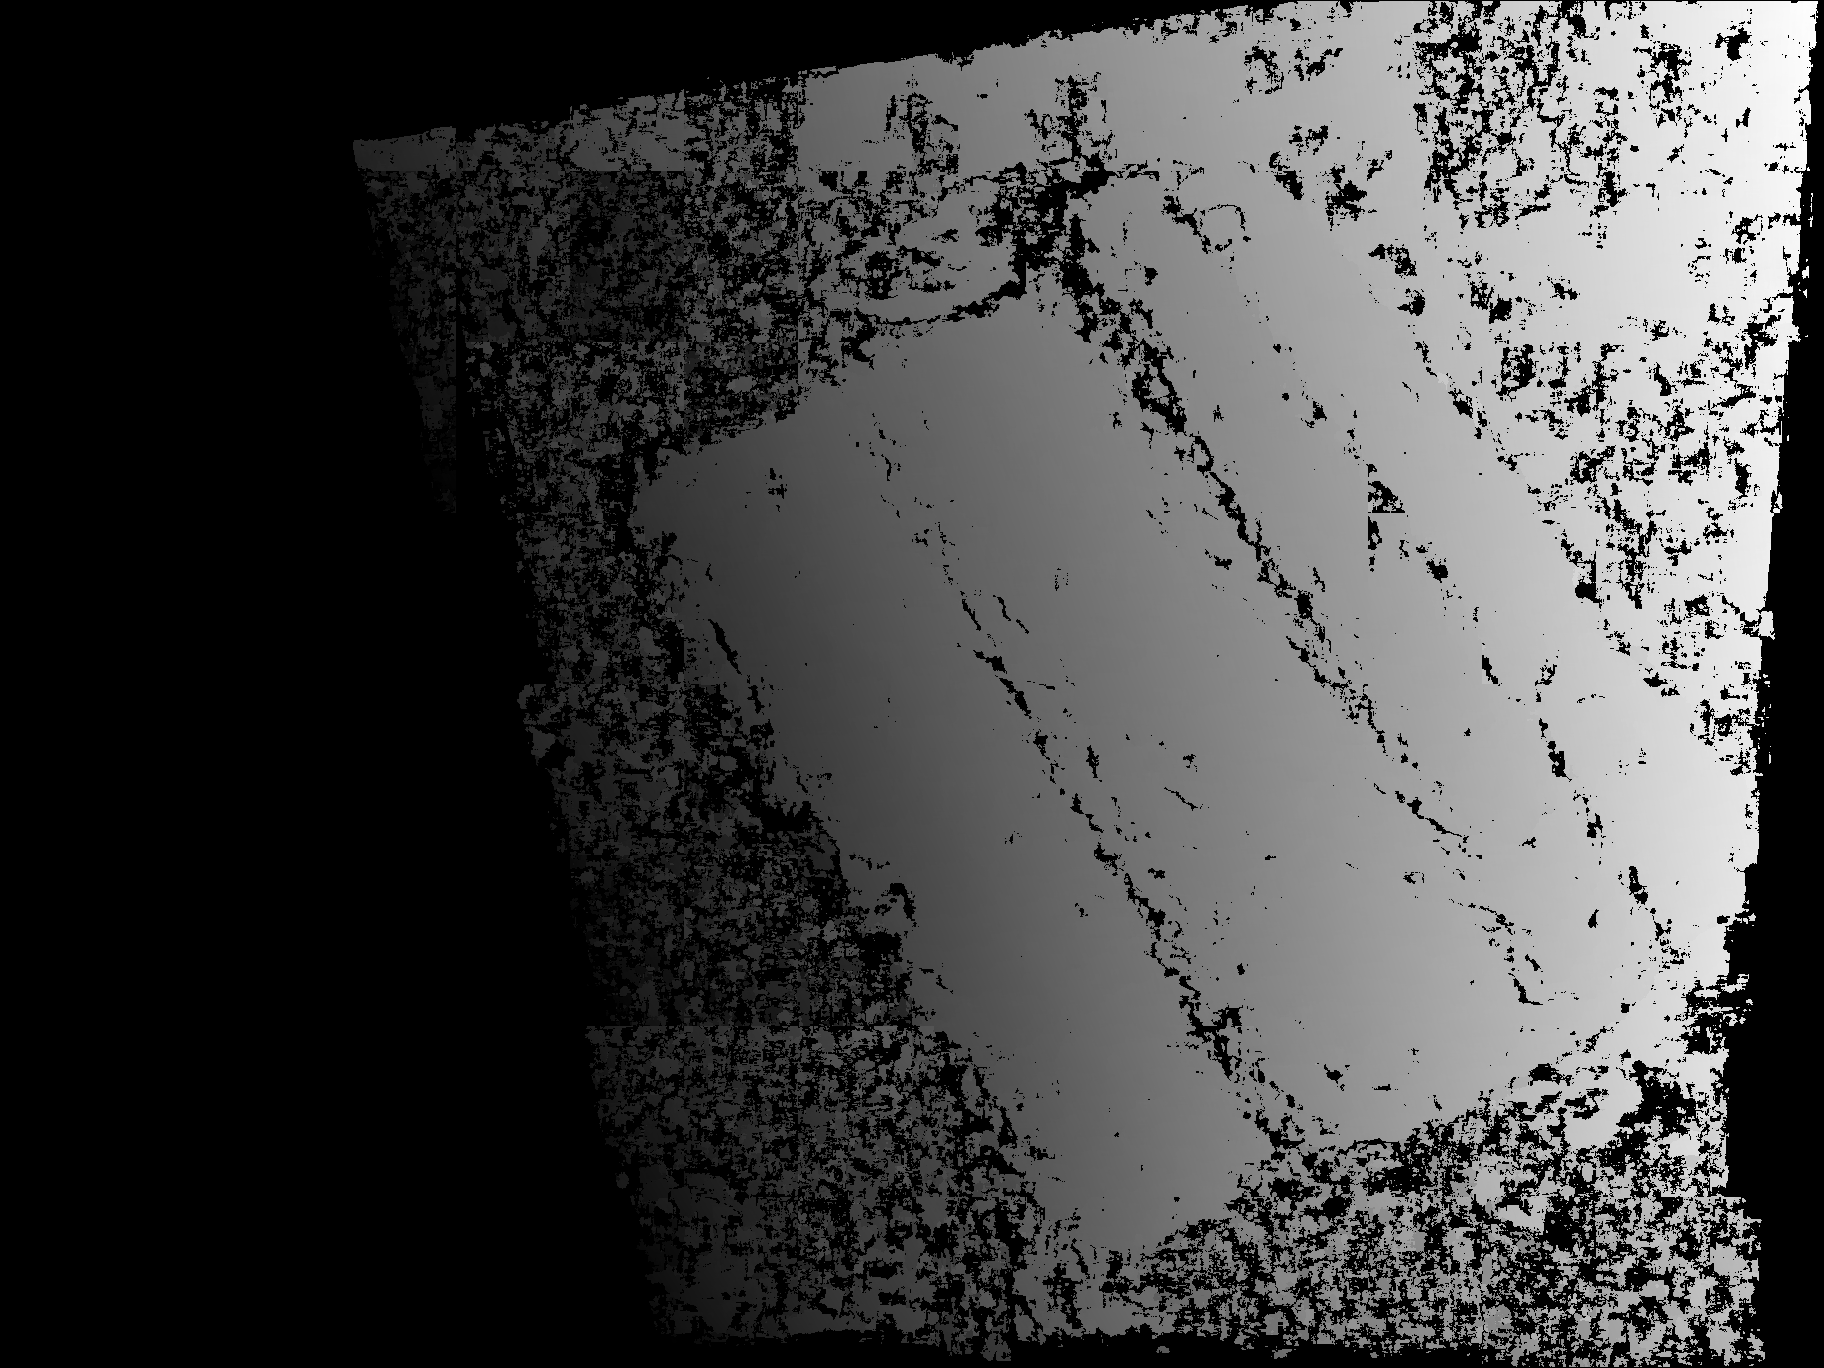
\includegraphics[width=4in]{images/stereo/y_disparity.png}\label{fig:disp-ex-ch1}}
\caption{Example of a Disparity Map created from pictures of a Sun Chip.}
\label{fig:disparity-example}
\end{figure}

The header file {\tt<vw/Stereo/DisparityMap.h>} provides a collection
of useful tools for working with and modifying disparities. Those
functions are listed in Table \ref{tbl:disparity-map-functions}. Tasks
that are not provided in the table are often possible with the generic
routines for working with {\tt PixelMasks}. For those abilities take
look back at Table \ref{tbl:pixel-mask-image-ops}.

\begin{table}[tbh]\begin{centering}
\begin{tabular}{|p{3 in}|p{4 in}|} \hline
Function & Description \\ \hline \hline
{\tt get\_disparity\_range(img)} & Returns a bounding box with a min \& max describing the value ranges of the disparity map \\ \hline
{\tt missing\_pixel\_image(img)} & Creates a new RGB image describing showing good pixel locations \\ \hline
{\tt disparity\_mask(disparity, Lmask, Rmask)} & Creates a new disparity map this valid only where the disparity links are valid in both the Left and Right images. {\tt Lmask} \& {\tt Rmask} are uint8 images where 255 is valid. \\ \hline
{\tt disparity\_range\_make(disparity, min, max)} & Invalidates pixel locations in a disparity map where the values exceed the values of {\tt min} \& {\tt max}. \\ \hline
{\tt remove\_outliers(disparity, half\_h\_kern, half\_v\_kern, p\_threshold, rej\_threshold)} & An erosion like method to take out high frequency changes in the disparity map and label them as invalid. \\ \hline
{\tt clean\_up(disparity, half\_h\_kern, half\_v\_kern)} & Applies {\tt remove\_outliers} twice with second application targeting single pixel outliers \\ \hline
{\tt std\_dev\_image(disparity, kern\_w, kern\_h)} & Remove pixels from the disparity map that correspond to low contrast pixels \\ \hline
{\tt transform\_disparities(disparity, trans)} & Applies a transform {\tt tans} to a disparity map \\ \hline
\end{tabular}
\caption{ Functions provided for working with Disparity Maps.}
\label{tbl:disparity-map-functions}
\end{centering}
\end{table}

Of the above functions, {\tt transform\_disparities} is of particular
interest. Before attempting to correlate to images it is best to do a
rough align for the images (like making sure both images are
upright). A transform can be solved for with interest points and then
applied to the right image. After solving for the disparity map
between the left and the transform right image, {\tt transform\_disparities}
can be applied to the disparity map with the inverse transform. Making
the disparity map correlate between the original left and right
images. This step of aligning the images before processing is
sometimes called rectification and it can play a big part in the
performance of stereo processing.

\section{Stereo Correlation}
\label{sec:stereo_correlation}

In this section we'll cover the techniques and the code to solve for a
disparity map with integer precision. First we'll start out with the
general idea of correlation. Then we'll break out in sections with
ways on how to speed of the process.

Correlation again is solving for a given point in the left image's
corresponding point in the right image. This is performed with
template matching.

\begin{figure}[h]
\begin{center}
  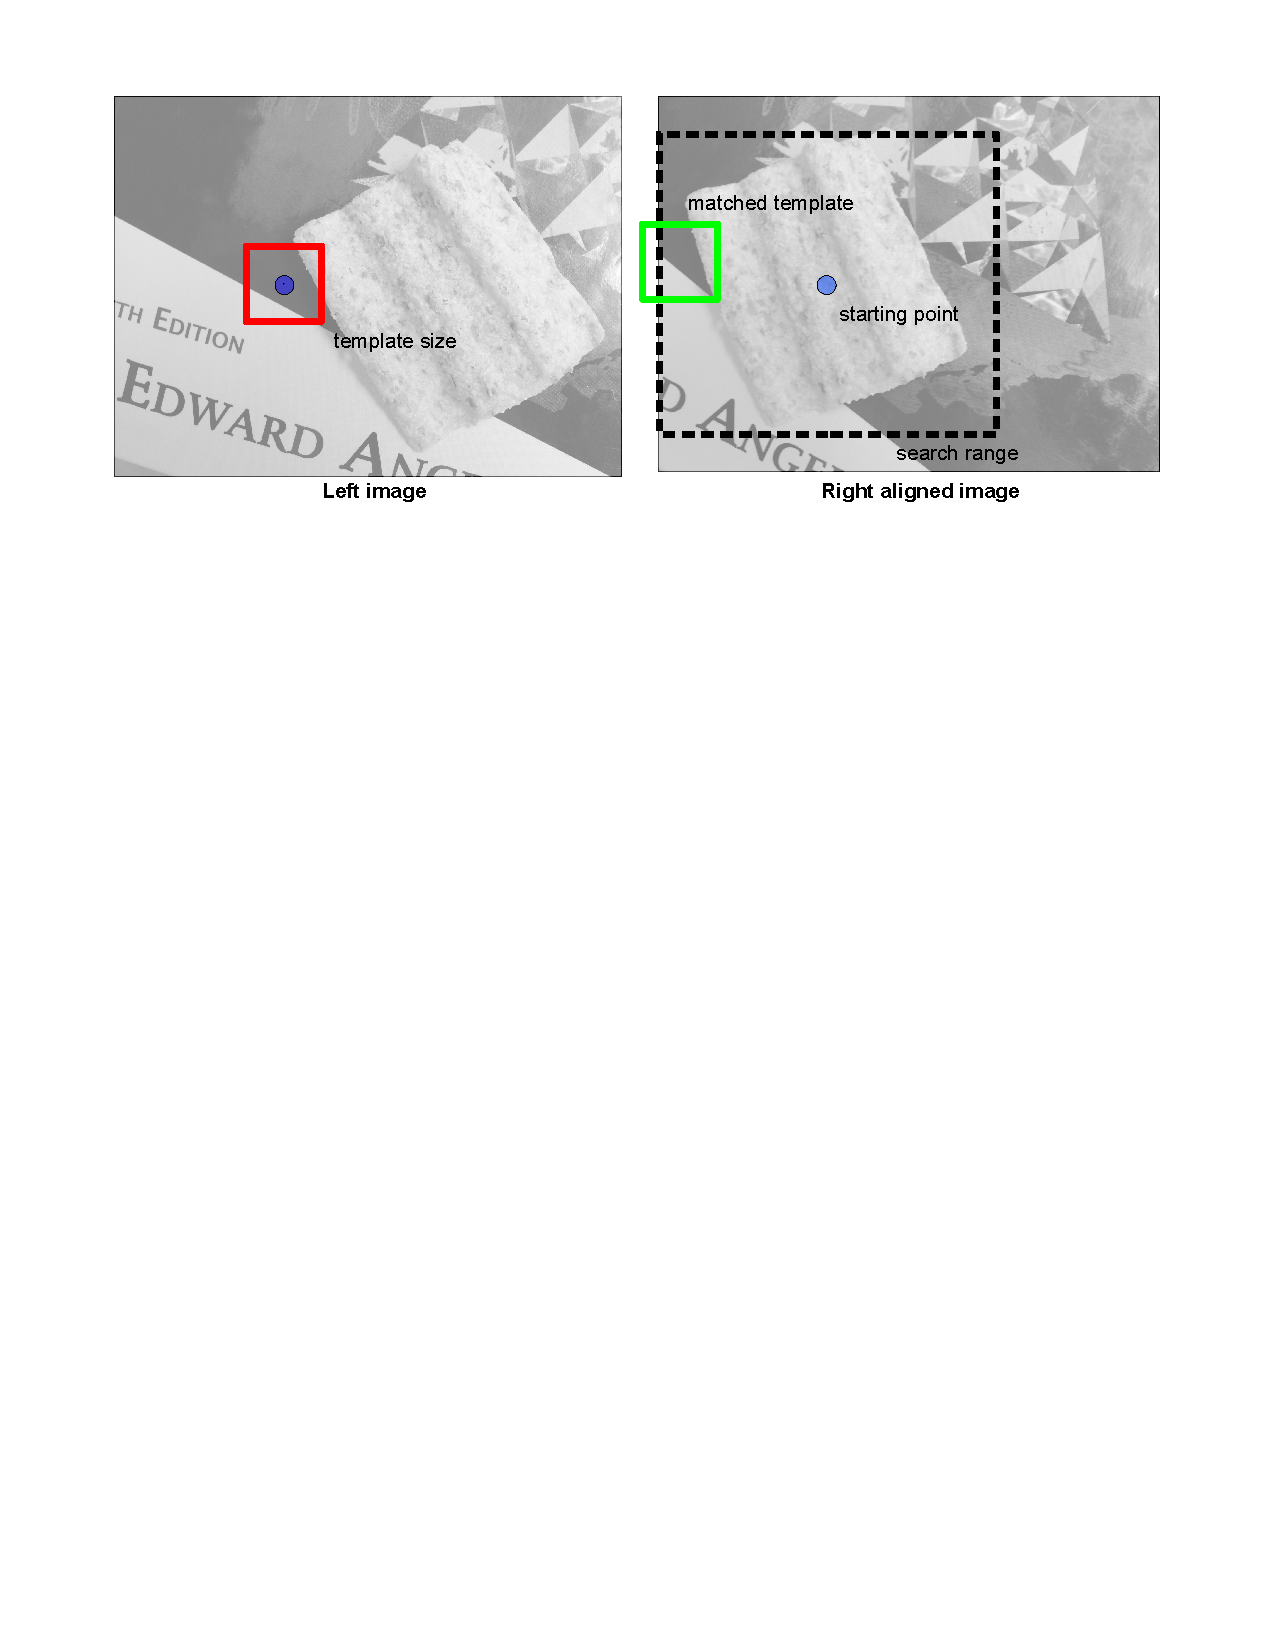
\includegraphics[trim = 0in 8in 0in 0in, width=6in]{images/stereo/template_matching.pdf}
\end{center}
  \caption{Template matching example}
  \label{fig:template_matching}
\end{figure}

Template matching is basically taking a crop of the image (called a
kernel) around a point in the left image and then trying to find a
similar point in the right image. A search range is defined for the
right image and a kernel is slid across the entire range. To determine
if a kernel position in the right image corresponds with the kernel in
the left image, a cost function is used. Normally we work with the sum
of absolute differences between the kernels, meaning that a low value
is high correlation and a high value means those kernels just don't
match. In our code we call this simply absolute difference. There are
other cost functions as well, squared difference and normalized cross
correlation. Yet all of them still boil down to per pixel difference
being calculated between the 2 kernels.

Stereo Module does the task of template matching most plainly in the
{\tt ReferenceCorrelator} found in {\tt <vw/Stereo/ReferenceCorrelator.h>}.
Yet this is not recommended for
general use, instead an better interface is provided called
{\tt CorrelatorView} found in {\tt <vw/Stereo/CorrelatorView.h>}. Here's an
example for implementing it.

\begin{verbatim}
  CorrelatorView<PixelGray<float>,vw::uint8,SlogStereoPreprocessingFilter>
    corr_view( left_disk_image, right_disk_image, left_mask, right_mask,
               SlogStereoPreprocessingFilter(1.5) );
  corr_view.set_search_range(search_range);
  corr_view.set_kernel_size(Vector2i(25,25));
  corr_view.set_correlator_options(1, ABS_DIFF_CORRELATOR);

  // Begin processing
  ImageView<PixelMask<Vector2f> > disparity_map = corr_view;
\end{verbatim}

That may seem like a lot of properties to set but don't let it
frighten you away. The original inputs are the 2 input images, 2 mask
images, and a preprocessing filter. Mask images are simply vw::uint8
images that are white where an image is valid. This is useful for
masking off objects that are known to cause problems before hand like
shadows, dust, or a certain someone who was accidentally touching the
lens during the shot. The preprocessing filter options are defined in
{\tt <vw/Stereo/Correlate.h>}. The LoG filters are useful for making the
correlator light invariant as it only see edges after it is
applied. LoG filters are also a recommended filter for when trying
out. Blur filter is recommended for only when working the normalized
cross correlation cost function in template matching.

\begin{table}[hbt]\begin{centering}
\begin{tabular}{|c|p{4 in}|} \hline
Function & Description \\ \hline \hline
\verb#SlogStereoPreprocessingFilter(arg)# & Sign of Laplacian of the Gaussian filter. Allows for efficient XOR comparisons. {\tt arg} is the gaussian sigma size. \\ \hline
\verb#LogStereoPreprocessingFilter(arg)# & Laplacian of Gaussian filter. {\tt arg} is the gaussian sigma size. \\ \hline
\verb#BlurStereoPreprocessingFilter(arg)# & Gaussian blur. {\tt arg} is the gaussian sigma size. \\ \hline
\verb#NullStereoPreprocessingFilter()# & No preprocessing. \\ \hline
\end{tabular}
\caption{Built-in preprocessing filter options.}
\label{tbl:preprocessing-filters}
\end{centering}\end{table}

One the other lines we set the search range with a bounding box. Where
origin of the bounding box is the starting search location in the
right image. Kernel size is the same as the template window's
size. Finally the correlator options sets kernel size for an
additional option blur that is applied internally and it sets the cost
function used in template matching. Table
\ref{tbl:correlator-cost-functions} has the available options for cost
functions.

\begin{table}[htb]\begin{centering}
\begin{tabular}{|c|p{4 in}|} \hline
Enumerator & Description \\ \hline \hline
\verb#ABS_DIFF_CORRELATOR# & Use the sum of absolute differences between paired kernels \\ \hline
\verb#SQR_DIFF_CORRELATOR# & Use the sum of squared differences between paired kernels \\ \hline
\verb#NORM_XCORR_CORRELATOR# & Normalized cross correlation cost function. \\ \hline
\end{tabular}
\caption{Correlator cost function options.}
\label{tbl:correlator-cost-functions}
\end{centering}\end{table}

This process of template matching is repeated for every pixel in the
left image against a search range in the right image. It should be
obvious why this is a CPU intensive process. Yet there are methods for
doing template matching efficiently and they are using a box filter
and by implementing a pyramid method to processing. The following
subsections cover those improvements, but it's not required reading as
{\tt CorrelatorView} implements them on default.

\subsection{Box-filter Optimized Correlator}

Here there be text

\begin{figure}[h]
\begin{center}
  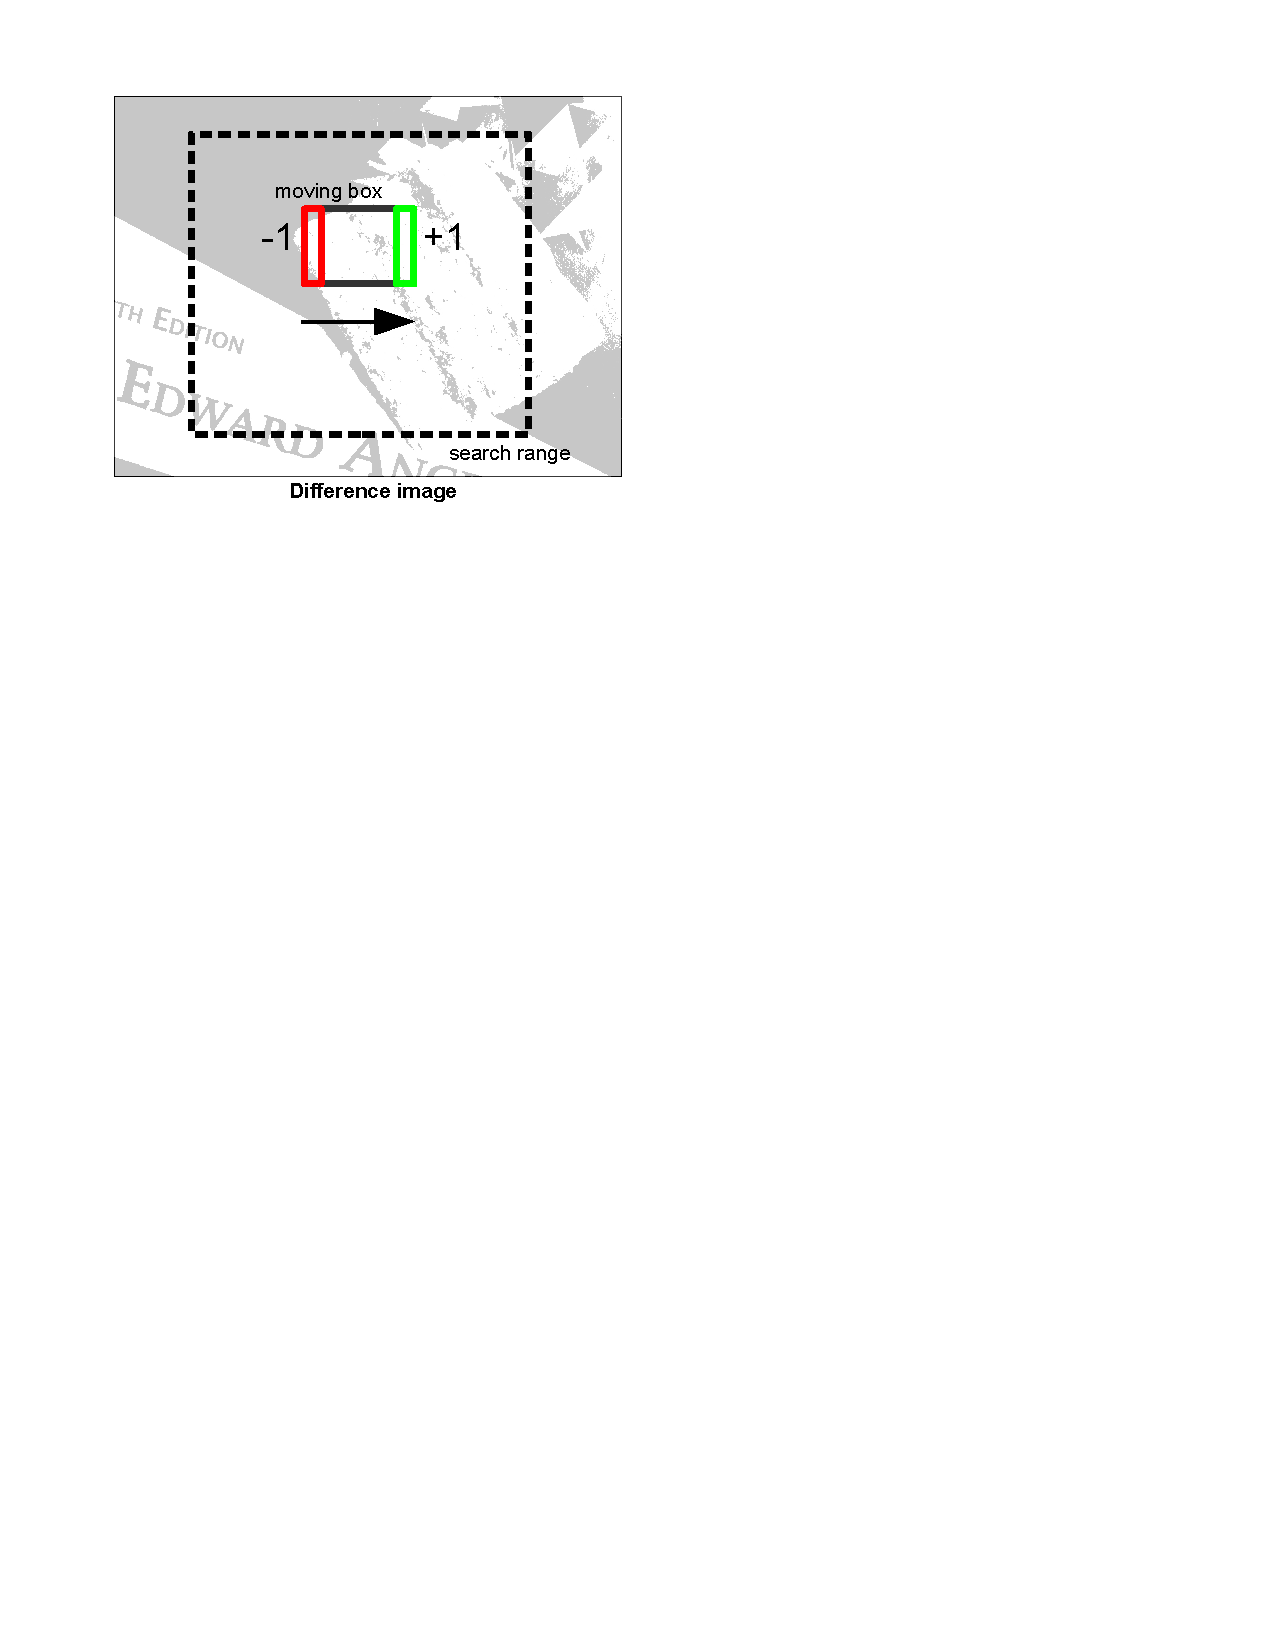
\includegraphics[trim = 0in 8in 3.5in 0in, width=3.75in]{images/stereo/boxfilter.pdf}
\end{center}
  \caption{Box filter Optimization}
  \label{fig:box_filter}
\end{figure}

Here there be text

\subsection{Pyramid-based Search Refinement}

Pyramid-based searches are pretty straight forward. Our first step is
producing a gaussian pyramid of the input images. This means
repeatedly blurring the image a small amount and then subsampling by
2. The highest level of the pyramid is the smallest image as it has
been subsampled the most. The top level is where we start our template
matching.

\begin{figure}[h]
\begin{center}
  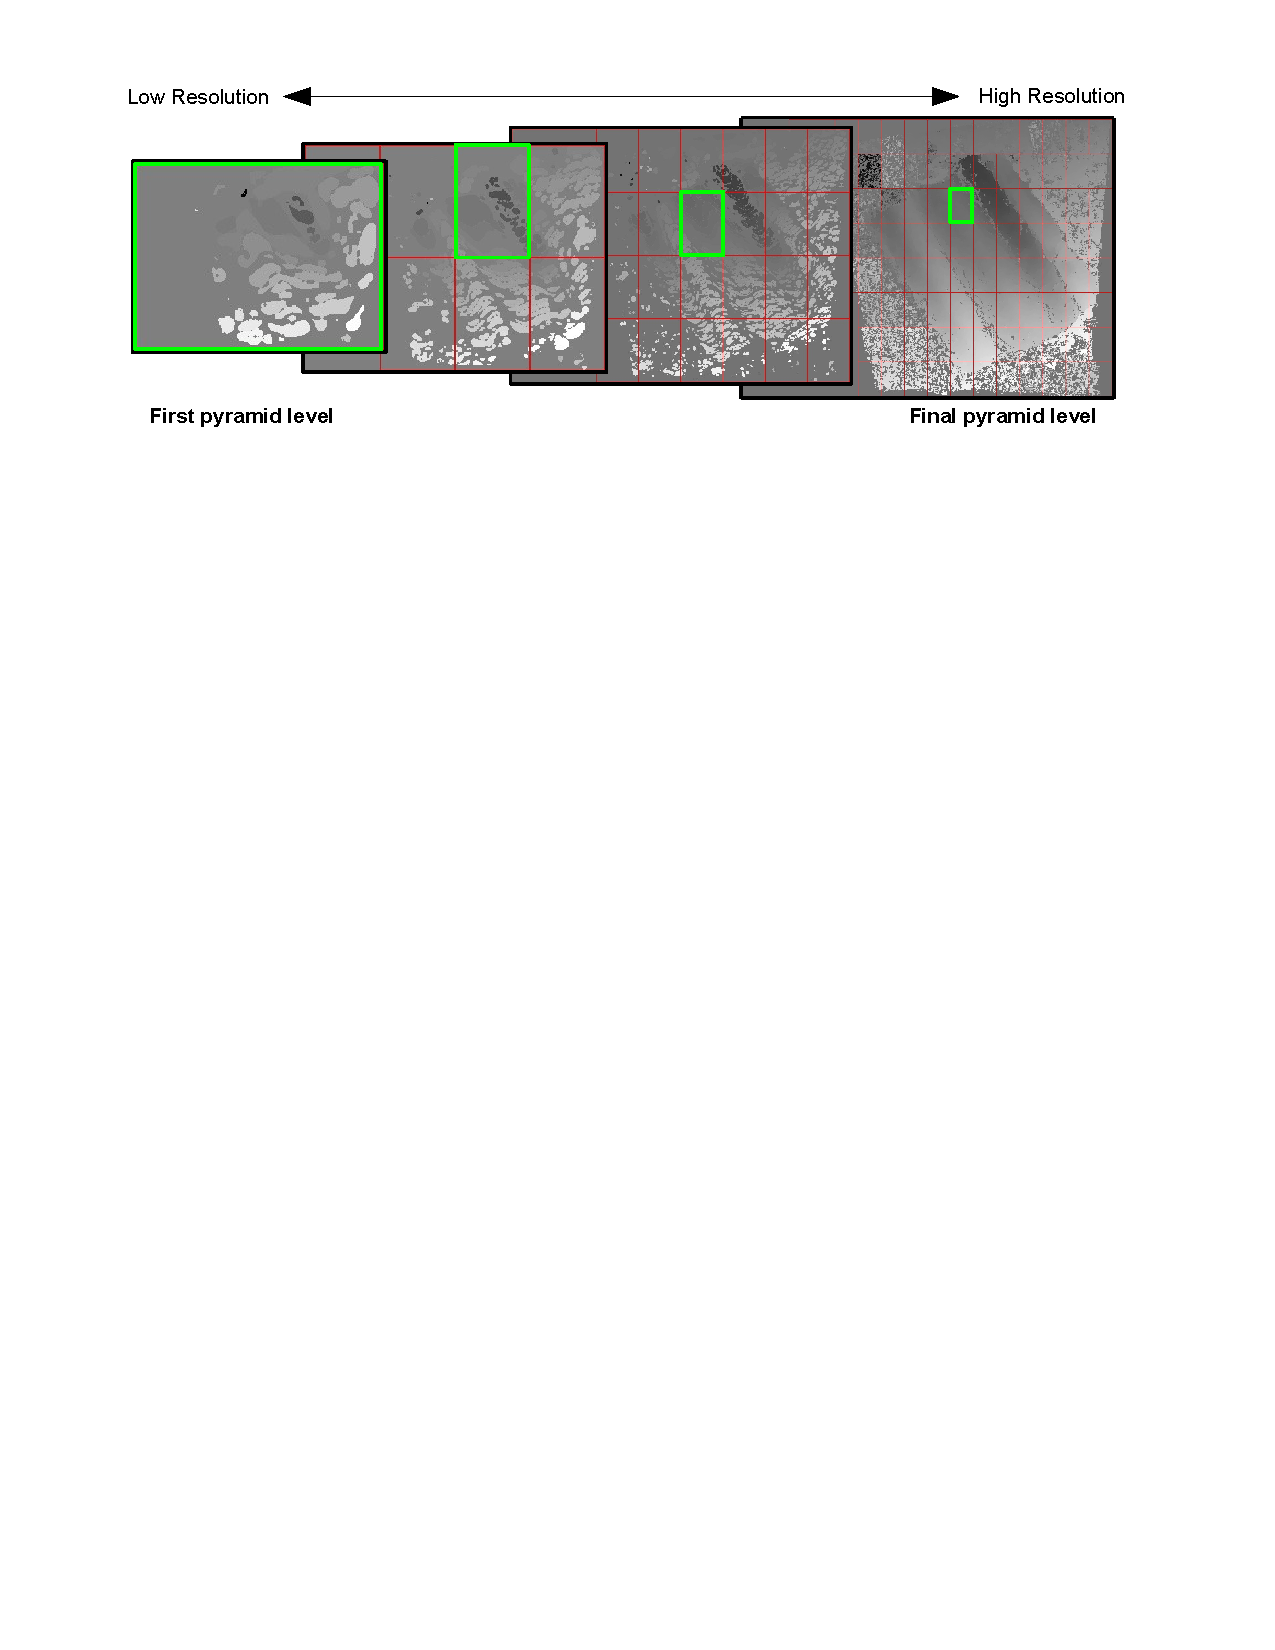
\includegraphics[trim = 0in 8.5in 0in 0in, width=7in]{images/stereo/pyramid_graphic.pdf}
\end{center}
  \caption{Pyramid-based search refinement}
  \label{fig:pyramid_search}
\end{figure}

From the top level our search range for the kernel has been reduced
greatly so it's processing time is very short. The disparity map
created with the reduced imagery is then used as a seed for the next
lower level of the pyramid. This is wonderful as the previous results
from a higher level will have the template window searching roughly in
the correct area and that means the search region is kept relatively
small. Using the pyramid search, each level is used as a seed for the
next lowest level until the bottom is reached. The result for the
lowest level is the disparity map for the original resolution imagery.

\section{Subpixel Refinement}
\label{sec:subpixel_refinement}

After disparity image is created with {\tt CorrelatorView}, it is very
coarse and exhibits what looks like stair steps in the 3D model. This
is because CorrelatorView has solved for the disparity using only
whole numbers. Subpixel Refinement further polishes the disparity map
into floating point precision. This additional step can be accessed
can be found in {\tt <vw/Stereo/SubpixelView.h>}.

\begin{verbatim}
disparity_map = SubpixelView<LogStereoPreprocessingFilter>(disparity_map_integer,
        left_image, right_image,
        25, 25,          // Kernel size
        true, true,      // Do H V subpixel
        0,               // Subpixel mode
        LogStereoPreprocessingFilter(1.5),
        false);          // Verbose option
\end{verbatim}

Above is an example of code using {\tt SubpixelView}. The first few
arguments should be pretty straight forward. It's the disparity map
created from {\tt CorrelatorView} and then the left and right original
images. The next two numbers are the kernel size to be used, these do
not need to be the same as what was used in integer correlation. After
that are two boolean conditionals that turn on horizontal and vertical
subpixel. Normally both of those values should be true. Yet for some
applications where speed is important, subpixel is only turned on for
one direction.

The last three are self explanatory except Subpixel mode. Stereo
module currently has 4 different sub pixel refinement algorithms and
with each increment they have better quality but at the cost of
speed. Mode 0 is parabola fitting and the fastest. It discussed in the
next subsection. Modes 1-3 are forms of affine kernel algorithms and
are discussed in the subsection \ref{sec:affine_subpixel}. Of these
modes, it is suggested starting out with Mode 0 and then when time is
not important jump directly to using Mode 3.

\begin{table}[htb]\begin{centering}
\begin{tabular}{|c|c|p{3.5 in}|} \hline
Mode & Name & Description \\ \hline \hline
0 & \verb#Parabola Subpixel# & Simplest and fastest subpixel mode. \\ \hline
1 & \verb#Robust Affine Subpixel# & Affine window subpixel with robust cost functions. \\ \hline
2 & \verb#Bayes Affine Subpixel# & Affine with gaussian weighted window. \\ \hline
3 & \verb#Bayes EM Affine Subpixel# & Affine with estimated parameters for gaussian weighted window\\ \hline
4 & \verb#Experimental Subpixel# & Affine with estimated parameters for gamma and gaussian weighted windows that correspond to inlier and outlier models\\ \hline
\end{tabular}
\caption{Available Subpixel modes.}
\label{tbl:subpixel-modes}
\end{centering}\end{table}

\subsection{Parabola Fitting in the Disparity Space Image}
\label{sec:parabola_subpixel}

\subsection{Affine-adaptive Subpixel Refinement}
\label{sec:affine_subpixel}

Text

\begin{figure}[h]
\begin{center}
  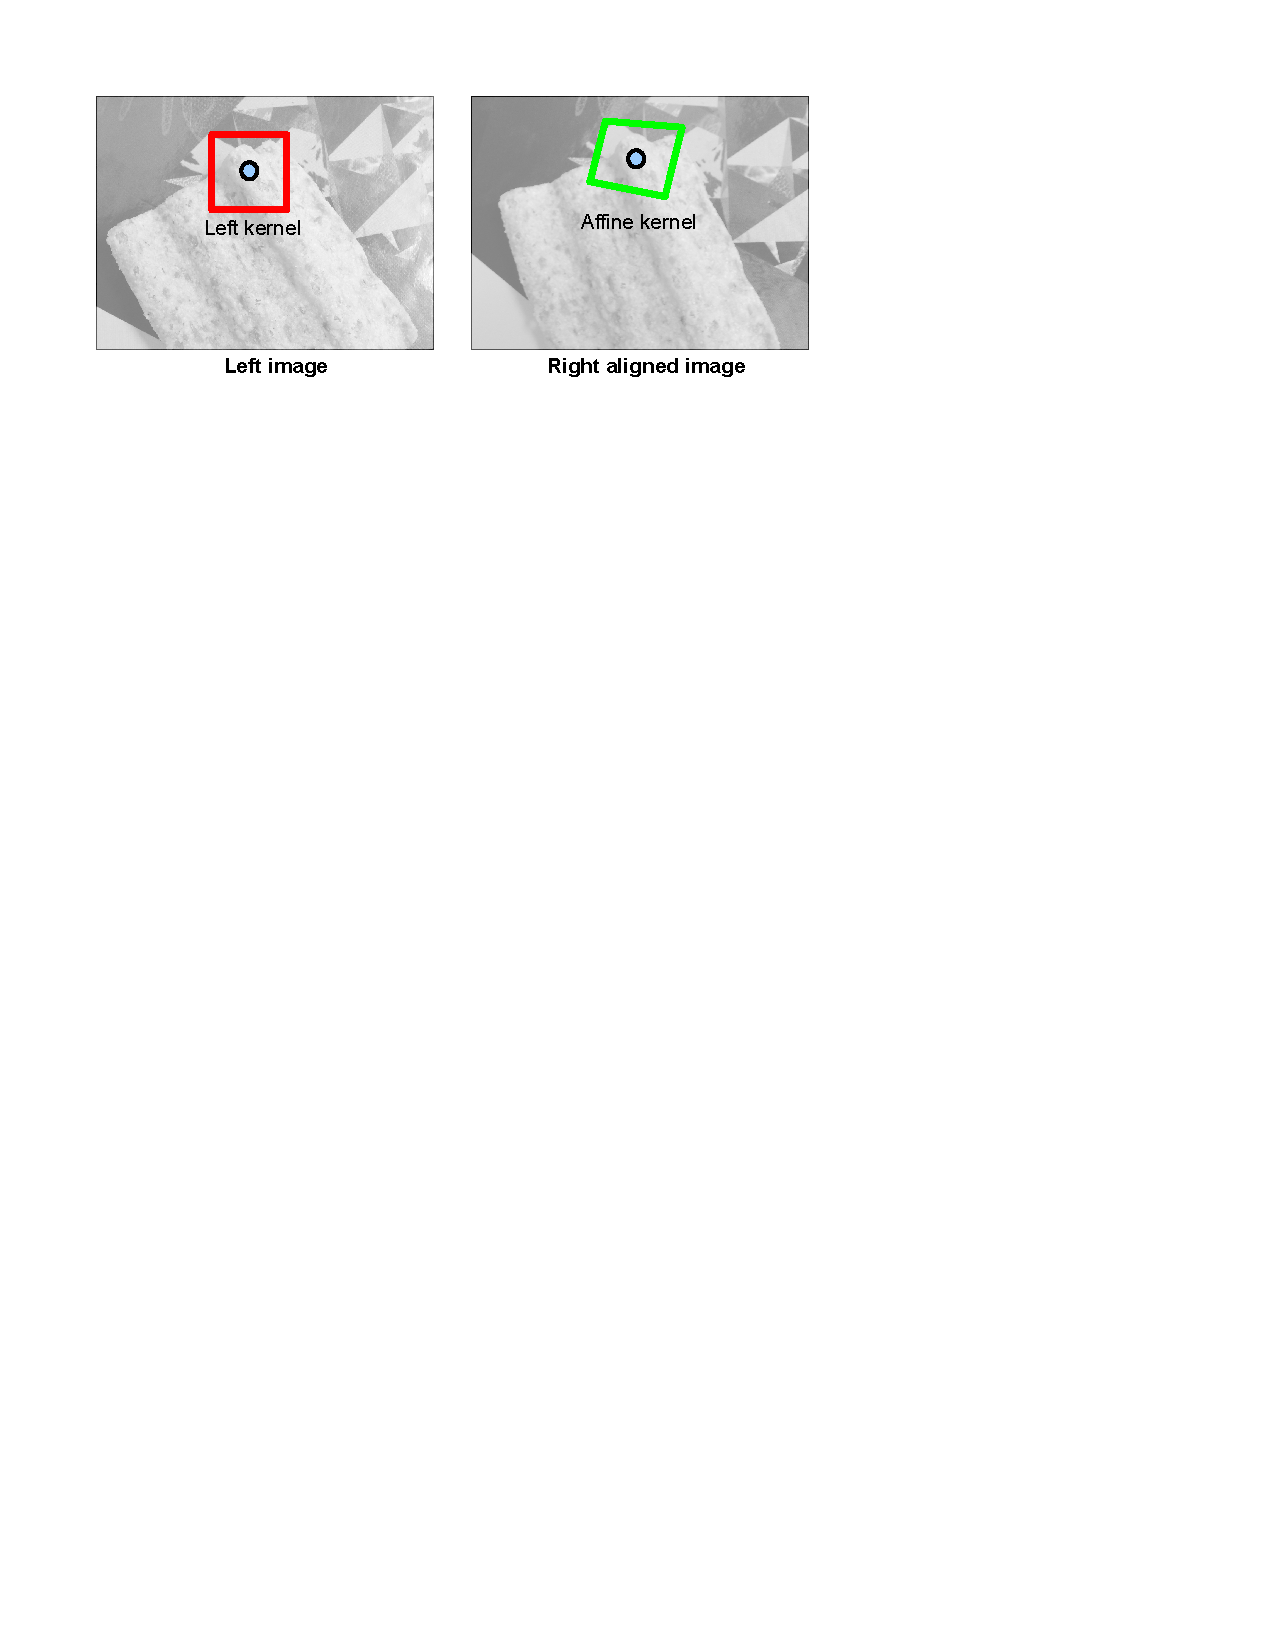
\includegraphics[trim = 0in 9in 3in 0in, width=4in]{images/stereo/affine_window.pdf}
\end{center}
  \caption{Affine refinement}
  \label{fig:affine_refinement}
\end{figure}

Text

%\subsection{Global Operators}

%\subsection{Local Operators}

\section{Point Clouds}
\label{sec:command_line_tools}

\section{Command Line Tool}
\label{sec:command_line_tool}

Vision Workbench only comes with one tool that uses the Stereo
Module. That is \verb#correlate# which can be read up in the Tools
Chapter in Section \ref{sec:correlate}. That tool is only a demo of
things possible and was used to create the imagery in this chapter. For
a more extreme example of what can be done with the stereo module, we
encourage you to check out the Ames Stereo Pipeline.

\begin{thebibliography}{1}

\end{thebibliography}
